\documentclass[1p]{elsarticle_modified}
%\bibliographystyle{elsarticle-num}

%\usepackage[colorlinks]{hyperref}
%\usepackage{abbrmath_seonhwa} %\Abb, \Ascr, \Acal ,\Abf, \Afrak
\usepackage{amsfonts}
\usepackage{amssymb}
\usepackage{amsmath}
\usepackage{amsthm}
\usepackage{scalefnt}
\usepackage{amsbsy}
\usepackage{kotex}
\usepackage{caption}
\usepackage{subfig}
\usepackage{color}
\usepackage{graphicx}
\usepackage{xcolor} %% white, black, red, green, blue, cyan, magenta, yellow
\usepackage{float}
\usepackage{setspace}
\usepackage{hyperref}

\usepackage{tikz}
\usetikzlibrary{arrows}

\usepackage{multirow}
\usepackage{array} % fixed length table
\usepackage{hhline}

%%%%%%%%%%%%%%%%%%%%%
\makeatletter
\renewcommand*\env@matrix[1][\arraystretch]{%
	\edef\arraystretch{#1}%
	\hskip -\arraycolsep
	\let\@ifnextchar\new@ifnextchar
	\array{*\c@MaxMatrixCols c}}
\makeatother %https://tex.stackexchange.com/questions/14071/how-can-i-increase-the-line-spacing-in-a-matrix
%%%%%%%%%%%%%%%

\usepackage[normalem]{ulem}

\newcommand{\msout}[1]{\ifmmode\text{\sout{\ensuremath{#1}}}\else\sout{#1}\fi}
%SOURCE: \msout is \stkout macro in https://tex.stackexchange.com/questions/20609/strikeout-in-math-mode

\newcommand{\cancel}[1]{
	\ifmmode
	{\color{red}\msout{#1}}
	\else
	{\color{red}\sout{#1}}
	\fi
}

\newcommand{\add}[1]{
	{\color{blue}\uwave{#1}}
}

\newcommand{\replace}[2]{
	\ifmmode
	{\color{red}\msout{#1}}{\color{blue}\uwave{#2}}
	\else
	{\color{red}\sout{#1}}{\color{blue}\uwave{#2}}
	\fi
}

\newcommand{\Sol}{\mathcal{S}} %segment
\newcommand{\D}{D} %diagram
\newcommand{\A}{\mathcal{A}} %arc


%%%%%%%%%%%%%%%%%%%%%%%%%%%%%5 test

\def\sl{\operatorname{\textup{SL}}(2,\Cbb)}
\def\psl{\operatorname{\textup{PSL}}(2,\Cbb)}
\def\quan{\mkern 1mu \triangleright \mkern 1mu}

\theoremstyle{definition}
\newtheorem{thm}{Theorem}[section]
\newtheorem{prop}[thm]{Proposition}
\newtheorem{lem}[thm]{Lemma}
\newtheorem{ques}[thm]{Question}
\newtheorem{cor}[thm]{Corollary}
\newtheorem{defn}[thm]{Definition}
\newtheorem{exam}[thm]{Example}
\newtheorem{rmk}[thm]{Remark}
\newtheorem{alg}[thm]{Algorithm}

\newcommand{\I}{\sqrt{-1}}
\begin{document}

%\begin{frontmatter}
%
%\title{Boundary parabolic representations of knots up to 8 crossings}
%
%%% Group authors per affiliation:
%\author{Yunhi Cho} 
%\address{Department of Mathematics, University of Seoul, Seoul, Korea}
%\ead{yhcho@uos.ac.kr}
%
%
%\author{Seonhwa Kim} %\fnref{s_kim}}
%\address{Center for Geometry and Physics, Institute for Basic Science, Pohang, 37673, Korea}
%\ead{ryeona17@ibs.re.kr}
%
%\author{Hyuk Kim}
%\address{Department of Mathematical Sciences, Seoul National University, Seoul 08826, Korea}
%\ead{hyukkim@snu.ac.kr}
%
%\author{Seokbeom Yoon}
%\address{Department of Mathematical Sciences, Seoul National University, Seoul, 08826,  Korea}
%\ead{sbyoon15@snu.ac.kr}
%
%\begin{abstract}
%We find all boundary parabolic representation of knots up to 8 crossings.
%
%\end{abstract}
%\begin{keyword}
%    \MSC[2010] 57M25 
%\end{keyword}
%
%\end{frontmatter}

%\linenumbers
%\tableofcontents
%
\newcommand\colored[1]{\textcolor{white}{\rule[-0.35ex]{0.8em}{1.4ex}}\kern-0.8em\color{red} #1}%
%\newcommand\colored[1]{\textcolor{white}{ #1}\kern-2.17ex	\textcolor{white}{ #1}\kern-1.81ex	\textcolor{white}{ #1}\kern-2.15ex\color{red}#1	}

{\Large $\underline{12n_{0720}~(K12n_{0720})}$}

\setlength{\tabcolsep}{10pt}
\renewcommand{\arraystretch}{1.6}
\vspace{1cm}\begin{tabular}{m{100pt}>{\centering\arraybackslash}m{274pt}}
\multirow{5}{120pt}{
	\centering
	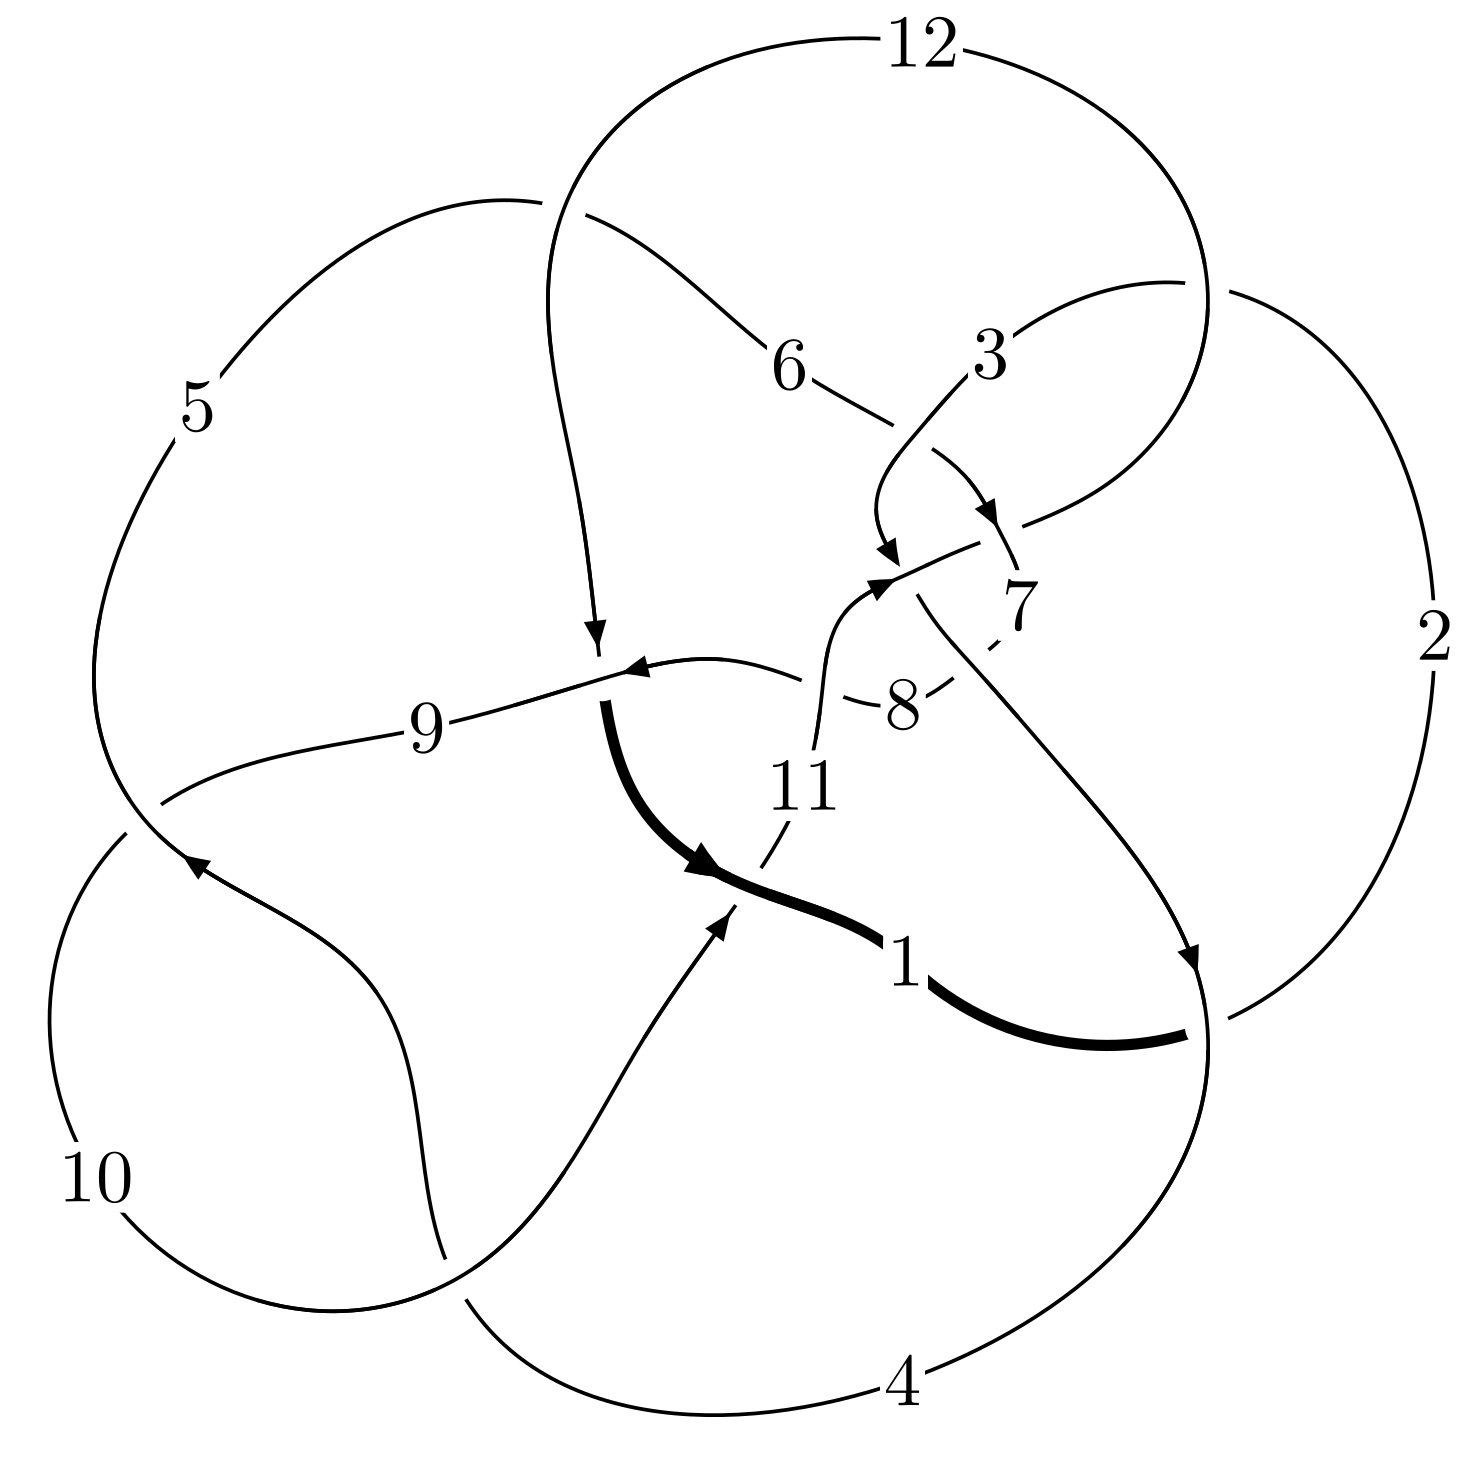
\includegraphics[width=112pt]{../../../GIT/diagram.site/Diagrams/png/2809_12n_0720.png}\\
\ \ \ A knot diagram\footnotemark}&
\allowdisplaybreaks
\textbf{Linearized knot diagam} \\
\cline{2-2}
 &
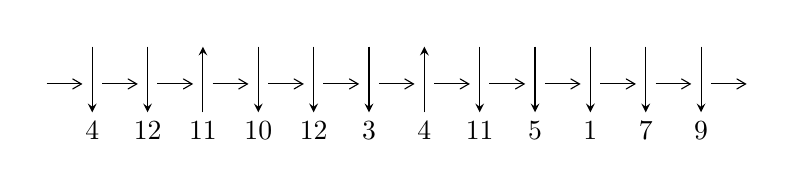
\begin{tikzpicture}[x=20pt, y=17pt]
	% nodes
	\node (C0) at (0, 0) {};
	\node (C1) at (1, 0) {};
	\node (C1U) at (1, +1) {};
	\node (C1D) at (1, -1) {4};

	\node (C2) at (2, 0) {};
	\node (C2U) at (2, +1) {};
	\node (C2D) at (2, -1) {12};

	\node (C3) at (3, 0) {};
	\node (C3U) at (3, +1) {};
	\node (C3D) at (3, -1) {11};

	\node (C4) at (4, 0) {};
	\node (C4U) at (4, +1) {};
	\node (C4D) at (4, -1) {10};

	\node (C5) at (5, 0) {};
	\node (C5U) at (5, +1) {};
	\node (C5D) at (5, -1) {12};

	\node (C6) at (6, 0) {};
	\node (C6U) at (6, +1) {};
	\node (C6D) at (6, -1) {3};

	\node (C7) at (7, 0) {};
	\node (C7U) at (7, +1) {};
	\node (C7D) at (7, -1) {4};

	\node (C8) at (8, 0) {};
	\node (C8U) at (8, +1) {};
	\node (C8D) at (8, -1) {11};

	\node (C9) at (9, 0) {};
	\node (C9U) at (9, +1) {};
	\node (C9D) at (9, -1) {5};

	\node (C10) at (10, 0) {};
	\node (C10U) at (10, +1) {};
	\node (C10D) at (10, -1) {1};

	\node (C11) at (11, 0) {};
	\node (C11U) at (11, +1) {};
	\node (C11D) at (11, -1) {7};

	\node (C12) at (12, 0) {};
	\node (C12U) at (12, +1) {};
	\node (C12D) at (12, -1) {9};
	\node (C13) at (13, 0) {};

	% arrows
	\draw[->,>={angle 60}]
	(C0) edge (C1) (C1) edge (C2) (C2) edge (C3) (C3) edge (C4) (C4) edge (C5) (C5) edge (C6) (C6) edge (C7) (C7) edge (C8) (C8) edge (C9) (C9) edge (C10) (C10) edge (C11) (C11) edge (C12) (C12) edge (C13) ;	\draw[->,>=stealth]
	(C1U) edge (C1D) (C2U) edge (C2D) (C3D) edge (C3U) (C4U) edge (C4D) (C5U) edge (C5D) (C6U) edge (C6D) (C7D) edge (C7U) (C8U) edge (C8D) (C9U) edge (C9D) (C10U) edge (C10D) (C11U) edge (C11D) (C12U) edge (C12D) ;
	\end{tikzpicture} \\
\hhline{~~} \\& 
\textbf{Solving Sequence} \\ \cline{2-2} 
 &
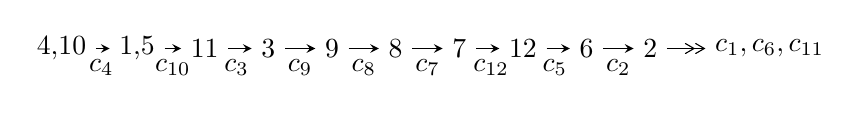
\begin{tikzpicture}[x=23pt, y=7pt]
	% node
	\node (A0) at (-1/8, 0) {4,10};
	\node (A1) at (17/16, 0) {1,5};
	\node (A2) at (17/8, 0) {11};
	\node (A3) at (25/8, 0) {3};
	\node (A4) at (33/8, 0) {9};
	\node (A5) at (41/8, 0) {8};
	\node (A6) at (49/8, 0) {7};
	\node (A7) at (57/8, 0) {12};
	\node (A8) at (65/8, 0) {6};
	\node (A9) at (73/8, 0) {2};
	\node (C1) at (1/2, -1) {$c_{4}$};
	\node (C2) at (13/8, -1) {$c_{10}$};
	\node (C3) at (21/8, -1) {$c_{3}$};
	\node (C4) at (29/8, -1) {$c_{9}$};
	\node (C5) at (37/8, -1) {$c_{8}$};
	\node (C6) at (45/8, -1) {$c_{7}$};
	\node (C7) at (53/8, -1) {$c_{12}$};
	\node (C8) at (61/8, -1) {$c_{5}$};
	\node (C9) at (69/8, -1) {$c_{2}$};
	\node (A10) at (11, 0) {$c_{1},c_{6},c_{11}$};

	% edge
	\draw[->,>=stealth]	
	(A0) edge (A1) (A1) edge (A2) (A2) edge (A3) (A3) edge (A4) (A4) edge (A5) (A5) edge (A6) (A6) edge (A7) (A7) edge (A8) (A8) edge (A9) ;
	\draw[->>,>={angle 60}]	
	(A9) edge (A10);
\end{tikzpicture} \\ 

\end{tabular} \\

\footnotetext{
The image of knot diagram is generated by the software ``\textbf{Draw programme}" developed by Andrew Bartholomew(\url{http://www.layer8.co.uk/maths/draw/index.htm\#Running-draw}), where we modified some parts for our purpose(\url{https://github.com/CATsTAILs/LinksPainter}).
}\phantom \\ \newline 
\centering \textbf{Ideals for irreducible components\footnotemark of $X_{\text{par}}$} 
 
\begin{align*}
I^u_{1}&=\langle 
-3.07560\times10^{132} u^{71}+1.26113\times10^{133} u^{70}+\cdots+2.19169\times10^{132} b+3.53314\times10^{134},\\
\phantom{I^u_{1}}&\phantom{= \langle  }-5.04578\times10^{133} u^{71}+1.39574\times10^{133} u^{70}+\cdots+3.72587\times10^{133} a+1.11463\times10^{135},\\
\phantom{I^u_{1}}&\phantom{= \langle  }u^{72}+24 u^{70}+\cdots+u+17\rangle \\
I^u_{2}&=\langle 
-6463690 u^{21}-7551941 u^{20}+\cdots+5470469 b-13759554,\\
\phantom{I^u_{2}}&\phantom{= \langle  }-16456196 u^{21}+170258 u^{20}+\cdots+5470469 a-12909429,\;u^{22}- u^{21}+\cdots-4 u+1\rangle \\
\\
\end{align*}
\raggedright * 2 irreducible components of $\dim_{\mathbb{C}}=0$, with total 94 representations.\\
\footnotetext{All coefficients of polynomials are rational numbers. But the coefficients are sometimes approximated in decimal forms when there is not enough margin.}
\newpage
\renewcommand{\arraystretch}{1}
\centering \section*{I. $I^u_{1}= \langle -3.08\times10^{132} u^{71}+1.26\times10^{133} u^{70}+\cdots+2.19\times10^{132} b+3.53\times10^{134},\;-5.05\times10^{133} u^{71}+1.40\times10^{133} u^{70}+\cdots+3.73\times10^{133} a+1.11\times10^{135},\;u^{72}+24 u^{70}+\cdots+u+17 \rangle$}
\flushleft \textbf{(i) Arc colorings}\\
\begin{tabular}{m{7pt} m{180pt} m{7pt} m{180pt} }
\flushright $a_{4}=$&$\begin{pmatrix}1\\0\end{pmatrix}$ \\
\flushright $a_{10}=$&$\begin{pmatrix}0\\u\end{pmatrix}$ \\
\flushright $a_{1}=$&$\begin{pmatrix}1.35425 u^{71}-0.374609 u^{70}+\cdots-0.0210176 u-29.9160\\1.40330 u^{71}-5.75416 u^{70}+\cdots-30.8710 u-161.206\end{pmatrix}$ \\
\flushright $a_{5}=$&$\begin{pmatrix}1\\u^2\end{pmatrix}$ \\
\flushright $a_{11}=$&$\begin{pmatrix}1.25553 u^{71}-0.745166 u^{70}+\cdots+19.7594 u-26.2435\\-1.91303 u^{71}-0.436232 u^{70}+\cdots-47.9897 u+4.43250\end{pmatrix}$ \\
\flushright $a_{3}=$&$\begin{pmatrix}-0.701200 u^{71}+0.0578726 u^{70}+\cdots+47.0698 u+38.4140\\1.03169 u^{71}+4.22675 u^{70}+\cdots+111.003 u+105.693\end{pmatrix}$ \\
\flushright $a_{9}=$&$\begin{pmatrix}u\\u^3+u\end{pmatrix}$ \\
\flushright $a_{8}=$&$\begin{pmatrix}-0.136773 u^{71}+0.391862 u^{70}+\cdots-1.59510 u+12.1738\\-3.37201 u^{71}-0.539374 u^{70}+\cdots-67.2143 u+17.8222\end{pmatrix}$ \\
\flushright $a_{7}=$&$\begin{pmatrix}3.23524 u^{71}+0.931236 u^{70}+\cdots+65.6192 u-5.64844\\-3.37201 u^{71}-0.539374 u^{70}+\cdots-67.2143 u+17.8222\end{pmatrix}$ \\
\flushright $a_{12}=$&$\begin{pmatrix}-0.364800 u^{71}+2.58232 u^{70}+\cdots-18.9166 u+51.2212\\1.51001 u^{71}-4.55294 u^{70}+\cdots-23.4995 u-130.337\end{pmatrix}$ \\
\flushright $a_{6}=$&$\begin{pmatrix}-2.19576 u^{71}+1.19016 u^{70}+\cdots-52.7840 u+45.5645\\1.33590 u^{71}-2.38359 u^{70}+\cdots+7.26507 u-84.1876\end{pmatrix}$ \\
\flushright $a_{2}=$&$\begin{pmatrix}-0.0490483 u^{71}+5.37955 u^{70}+\cdots+30.8499 u+131.290\\1.40330 u^{71}-5.75416 u^{70}+\cdots-30.8710 u-161.206\end{pmatrix}$\\&\end{tabular}
\flushleft \textbf{(ii) Obstruction class $= -1$}\\~\\
\flushleft \textbf{(iii) Cusp Shapes $= -10.1241 u^{71}+9.90473 u^{70}+\cdots-214.226 u+268.653$}\\~\\
\newpage\renewcommand{\arraystretch}{1}
\flushleft \textbf{(iv) u-Polynomials at the component}\newline \\
\begin{tabular}{m{50pt}|m{274pt}}
Crossings & \hspace{64pt}u-Polynomials at each crossing \\
\hline $$\begin{aligned}c_{1}\end{aligned}$$&$\begin{aligned}
&u^{72}-9 u^{71}+\cdots+1961 u-77
\end{aligned}$\\
\hline $$\begin{aligned}c_{2}\end{aligned}$$&$\begin{aligned}
&u^{72}+10 u^{71}+\cdots-907019 u-119125
\end{aligned}$\\
\hline $$\begin{aligned}c_{3}\end{aligned}$$&$\begin{aligned}
&u^{72}+2 u^{71}+\cdots+60020 u+6341
\end{aligned}$\\
\hline $$\begin{aligned}c_{4},c_{9}\end{aligned}$$&$\begin{aligned}
&u^{72}+24 u^{70}+\cdots+u+17
\end{aligned}$\\
\hline $$\begin{aligned}c_{5}\end{aligned}$$&$\begin{aligned}
&u^{72}-21 u^{70}+\cdots+35839731 u-10044233
\end{aligned}$\\
\hline $$\begin{aligned}c_{6}\end{aligned}$$&$\begin{aligned}
&u^{72}+4 u^{71}+\cdots+28820 u+2887
\end{aligned}$\\
\hline $$\begin{aligned}c_{7}\end{aligned}$$&$\begin{aligned}
&u^{72}-4 u^{71}+\cdots+157706 u+75839
\end{aligned}$\\
\hline $$\begin{aligned}c_{8}\end{aligned}$$&$\begin{aligned}
&u^{72}-17 u^{71}+\cdots-149942054 u+20559187
\end{aligned}$\\
\hline $$\begin{aligned}c_{10}\end{aligned}$$&$\begin{aligned}
&u^{72}- u^{71}+\cdots+7 u-1
\end{aligned}$\\
\hline $$\begin{aligned}c_{11}\end{aligned}$$&$\begin{aligned}
&u^{72}+3 u^{71}+\cdots-12 u+1
\end{aligned}$\\
\hline $$\begin{aligned}c_{12}\end{aligned}$$&$\begin{aligned}
&u^{72}+u^{71}+\cdots+865 u-575
\end{aligned}$\\
\hline
\end{tabular}\\~\\
\newpage\renewcommand{\arraystretch}{1}
\flushleft \textbf{(v) Riley Polynomials at the component}\newline \\
\begin{tabular}{m{50pt}|m{274pt}}
Crossings & \hspace{64pt}Riley Polynomials at each crossing \\
\hline $$\begin{aligned}c_{1}\end{aligned}$$&$\begin{aligned}
&y^{72}-29 y^{71}+\cdots-1058891 y+5929
\end{aligned}$\\
\hline $$\begin{aligned}c_{2}\end{aligned}$$&$\begin{aligned}
&y^{72}-78 y^{71}+\cdots+24427750639 y+14190765625
\end{aligned}$\\
\hline $$\begin{aligned}c_{3}\end{aligned}$$&$\begin{aligned}
&y^{72}+78 y^{71}+\cdots-240503656 y+40208281
\end{aligned}$\\
\hline $$\begin{aligned}c_{4},c_{9}\end{aligned}$$&$\begin{aligned}
&y^{72}+48 y^{71}+\cdots+6051 y+289
\end{aligned}$\\
\hline $$\begin{aligned}c_{5}\end{aligned}$$&$\begin{aligned}
&y^{72}-42 y^{71}+\cdots-2956824736496503 y+100886616558289
\end{aligned}$\\
\hline $$\begin{aligned}c_{6}\end{aligned}$$&$\begin{aligned}
&y^{72}-74 y^{71}+\cdots-527457400 y+8334769
\end{aligned}$\\
\hline $$\begin{aligned}c_{7}\end{aligned}$$&$\begin{aligned}
&y^{72}+90 y^{71}+\cdots-90986257534 y+5751553921
\end{aligned}$\\
\hline $$\begin{aligned}c_{8}\end{aligned}$$&$\begin{aligned}
&y^{72}-71 y^{71}+\cdots-12442914146716706 y+422680170100969
\end{aligned}$\\
\hline $$\begin{aligned}c_{10}\end{aligned}$$&$\begin{aligned}
&y^{72}- y^{71}+\cdots-7 y+1
\end{aligned}$\\
\hline $$\begin{aligned}c_{11}\end{aligned}$$&$\begin{aligned}
&y^{72}+5 y^{71}+\cdots-44 y+1
\end{aligned}$\\
\hline $$\begin{aligned}c_{12}\end{aligned}$$&$\begin{aligned}
&y^{72}-5 y^{71}+\cdots-2688275 y+330625
\end{aligned}$\\
\hline
\end{tabular}\\~\\
\newpage\flushleft \textbf{(vi) Complex Volumes and Cusp Shapes}
$$\begin{array}{c|c|c}  
\text{Solutions to }I^u_{1}& \I (\text{vol} + \sqrt{-1}CS) & \text{Cusp shape}\\
 \hline 
\begin{aligned}
u &= -0.477362 + 0.897642 I \\
a &= -0.067877 - 0.313856 I \\
b &= -1.151550 - 0.136492 I\end{aligned}
 & -1.61428 + 1.42833 I & \phantom{-0.000000 } 0 \\ \hline\begin{aligned}
u &= -0.477362 - 0.897642 I \\
a &= -0.067877 + 0.313856 I \\
b &= -1.151550 + 0.136492 I\end{aligned}
 & -1.61428 - 1.42833 I & \phantom{-0.000000 } 0 \\ \hline\begin{aligned}
u &= \phantom{-}0.315889 + 0.926424 I \\
a &= \phantom{-}0.432112 - 0.805014 I \\
b &= \phantom{-}1.14826 + 2.39805 I\end{aligned}
 & -6.56364 + 2.44744 I & \phantom{-0.000000 } 0 \\ \hline\begin{aligned}
u &= \phantom{-}0.315889 - 0.926424 I \\
a &= \phantom{-}0.432112 + 0.805014 I \\
b &= \phantom{-}1.14826 - 2.39805 I\end{aligned}
 & -6.56364 - 2.44744 I & \phantom{-0.000000 } 0 \\ \hline\begin{aligned}
u &= \phantom{-}0.133880 + 0.943058 I \\
a &= -0.707754 + 1.162790 I \\
b &= -0.66351 - 1.47027 I\end{aligned}
 & -0.37726 - 3.40325 I & -4.42658 + 3.83460 I \\ \hline\begin{aligned}
u &= \phantom{-}0.133880 - 0.943058 I \\
a &= -0.707754 - 1.162790 I \\
b &= -0.66351 + 1.47027 I\end{aligned}
 & -0.37726 + 3.40325 I & -4.42658 - 3.83460 I \\ \hline\begin{aligned}
u &= \phantom{-}0.301550 + 0.900946 I \\
a &= -0.147062 + 1.390830 I \\
b &= -0.742542 - 0.916719 I\end{aligned}
 & -2.08548 - 1.83389 I & -10.93305 + 0. I\phantom{ +0.000000I} \\ \hline\begin{aligned}
u &= \phantom{-}0.301550 - 0.900946 I \\
a &= -0.147062 - 1.390830 I \\
b &= -0.742542 + 0.916719 I\end{aligned}
 & -2.08548 + 1.83389 I & -10.93305 + 0. I\phantom{ +0.000000I} \\ \hline\begin{aligned}
u &= -0.215828 + 1.034000 I \\
a &= -1.77643 - 0.46095 I \\
b &= -0.933208 + 0.211167 I\end{aligned}
 & \phantom{-}3.17186 + 2.86604 I & \phantom{-0.000000 } 0 \\ \hline\begin{aligned}
u &= -0.215828 - 1.034000 I \\
a &= -1.77643 + 0.46095 I \\
b &= -0.933208 - 0.211167 I\end{aligned}
 & \phantom{-}3.17186 - 2.86604 I & \phantom{-0.000000 } 0\\
 \hline 
 \end{array}$$\newpage$$\begin{array}{c|c|c}  
\text{Solutions to }I^u_{1}& \I (\text{vol} + \sqrt{-1}CS) & \text{Cusp shape}\\
 \hline 
\begin{aligned}
u &= \phantom{-}0.377147 + 1.000300 I \\
a &= -0.60630 - 1.79537 I \\
b &= \phantom{-}0.491494 + 0.082853 I\end{aligned}
 & -6.71932 - 7.41916 I & \phantom{-0.000000 } 0 \\ \hline\begin{aligned}
u &= \phantom{-}0.377147 - 1.000300 I \\
a &= -0.60630 + 1.79537 I \\
b &= \phantom{-}0.491494 - 0.082853 I\end{aligned}
 & -6.71932 + 7.41916 I & \phantom{-0.000000 } 0 \\ \hline\begin{aligned}
u &= -0.433501 + 0.982102 I \\
a &= -0.464224 - 0.505661 I \\
b &= -0.40071 + 1.38684 I\end{aligned}
 & \phantom{-}0.19065 + 4.37559 I & \phantom{-0.000000 } 0 \\ \hline\begin{aligned}
u &= -0.433501 - 0.982102 I \\
a &= -0.464224 + 0.505661 I \\
b &= -0.40071 - 1.38684 I\end{aligned}
 & \phantom{-}0.19065 - 4.37559 I & \phantom{-0.000000 } 0 \\ \hline\begin{aligned}
u &= -0.502019 + 0.960993 I \\
a &= -0.38438 + 1.51469 I \\
b &= \phantom{-}0.472013 + 0.149646 I\end{aligned}
 & -6.73385 - 0.03465 I & \phantom{-0.000000 } 0 \\ \hline\begin{aligned}
u &= -0.502019 - 0.960993 I \\
a &= -0.38438 - 1.51469 I \\
b &= \phantom{-}0.472013 - 0.149646 I\end{aligned}
 & -6.73385 + 0.03465 I & \phantom{-0.000000 } 0 \\ \hline\begin{aligned}
u &= -0.871305 + 0.250604 I \\
a &= -1.134100 + 0.159082 I \\
b &= -0.910776 + 1.001180 I\end{aligned}
 & -3.47313 + 3.50227 I & -18.3256 - 7.5930 I \\ \hline\begin{aligned}
u &= -0.871305 - 0.250604 I \\
a &= -1.134100 - 0.159082 I \\
b &= -0.910776 - 1.001180 I\end{aligned}
 & -3.47313 - 3.50227 I & -18.3256 + 7.5930 I \\ \hline\begin{aligned}
u &= -1.101040 + 0.158588 I \\
a &= \phantom{-}0.860403 + 0.773355 I \\
b &= \phantom{-}1.230070 + 0.481564 I\end{aligned}
 & -10.34360 - 2.43121 I & \phantom{-0.000000 } 0 \\ \hline\begin{aligned}
u &= -1.101040 - 0.158588 I \\
a &= \phantom{-}0.860403 - 0.773355 I \\
b &= \phantom{-}1.230070 - 0.481564 I\end{aligned}
 & -10.34360 + 2.43121 I & \phantom{-0.000000 } 0\\
 \hline 
 \end{array}$$\newpage$$\begin{array}{c|c|c}  
\text{Solutions to }I^u_{1}& \I (\text{vol} + \sqrt{-1}CS) & \text{Cusp shape}\\
 \hline 
\begin{aligned}
u &= \phantom{-}1.027610 + 0.439052 I \\
a &= -0.144621 + 0.779286 I \\
b &= -0.540452 + 0.832986 I\end{aligned}
 & -1.51227 + 2.95975 I & \phantom{-0.000000 } 0 \\ \hline\begin{aligned}
u &= \phantom{-}1.027610 - 0.439052 I \\
a &= -0.144621 - 0.779286 I \\
b &= -0.540452 - 0.832986 I\end{aligned}
 & -1.51227 - 2.95975 I & \phantom{-0.000000 } 0 \\ \hline\begin{aligned}
u &= -0.298638 + 1.108140 I \\
a &= \phantom{-}0.589128 + 0.524624 I \\
b &= \phantom{-}1.68842 - 2.24180 I\end{aligned}
 & -4.91427 + 6.35505 I & \phantom{-0.000000 } 0 \\ \hline\begin{aligned}
u &= -0.298638 - 1.108140 I \\
a &= \phantom{-}0.589128 - 0.524624 I \\
b &= \phantom{-}1.68842 + 2.24180 I\end{aligned}
 & -4.91427 - 6.35505 I & \phantom{-0.000000 } 0 \\ \hline\begin{aligned}
u &= \phantom{-}0.461914 + 1.060090 I \\
a &= -1.41949 + 0.47743 I \\
b &= -1.32124 - 0.96303 I\end{aligned}
 & -1.40577 - 6.31505 I & \phantom{-0.000000 } 0 \\ \hline\begin{aligned}
u &= \phantom{-}0.461914 - 1.060090 I \\
a &= -1.41949 - 0.47743 I \\
b &= -1.32124 + 0.96303 I\end{aligned}
 & -1.40577 + 6.31505 I & \phantom{-0.000000 } 0 \\ \hline\begin{aligned}
u &= \phantom{-}1.158870 + 0.142308 I \\
a &= \phantom{-}0.786009 - 0.769271 I \\
b &= \phantom{-}1.173780 - 0.714165 I\end{aligned}
 & -10.2439 + 10.5771 I & \phantom{-0.000000 } 0 \\ \hline\begin{aligned}
u &= \phantom{-}1.158870 - 0.142308 I \\
a &= \phantom{-}0.786009 + 0.769271 I \\
b &= \phantom{-}1.173780 + 0.714165 I\end{aligned}
 & -10.2439 - 10.5771 I & \phantom{-0.000000 } 0 \\ \hline\begin{aligned}
u &= -0.091289 + 0.794865 I \\
a &= \phantom{-}1.00922 - 1.97778 I \\
b &= -0.130734 + 0.316777 I\end{aligned}
 & \phantom{-}2.12580 - 1.30198 I & -4.55096 - 6.52596 I \\ \hline\begin{aligned}
u &= -0.091289 - 0.794865 I \\
a &= \phantom{-}1.00922 + 1.97778 I \\
b &= -0.130734 - 0.316777 I\end{aligned}
 & \phantom{-}2.12580 + 1.30198 I & -4.55096 + 6.52596 I\\
 \hline 
 \end{array}$$\newpage$$\begin{array}{c|c|c}  
\text{Solutions to }I^u_{1}& \I (\text{vol} + \sqrt{-1}CS) & \text{Cusp shape}\\
 \hline 
\begin{aligned}
u &= \phantom{-}0.249808 + 1.185040 I \\
a &= \phantom{-}0.975289 - 0.228857 I \\
b &= \phantom{-}0.368779 + 0.841330 I\end{aligned}
 & \phantom{-}3.99365 + 0.15429 I & \phantom{-0.000000 } 0 \\ \hline\begin{aligned}
u &= \phantom{-}0.249808 - 1.185040 I \\
a &= \phantom{-}0.975289 + 0.228857 I \\
b &= \phantom{-}0.368779 - 0.841330 I\end{aligned}
 & \phantom{-}3.99365 - 0.15429 I & \phantom{-0.000000 } 0 \\ \hline\begin{aligned}
u &= \phantom{-}0.120517 + 0.770120 I \\
a &= -0.162776 - 0.214456 I \\
b &= \phantom{-}3.44943 - 0.72600 I\end{aligned}
 & -7.47162 - 4.79394 I & -20.2086 + 8.5185 I \\ \hline\begin{aligned}
u &= \phantom{-}0.120517 - 0.770120 I \\
a &= -0.162776 + 0.214456 I \\
b &= \phantom{-}3.44943 + 0.72600 I\end{aligned}
 & -7.47162 + 4.79394 I & -20.2086 - 8.5185 I \\ \hline\begin{aligned}
u &= \phantom{-}0.620042 + 0.447810 I \\
a &= -0.64813 + 1.64366 I \\
b &= -0.950767 + 0.538188 I\end{aligned}
 & -3.27579 + 2.08206 I & -17.7678 - 0.3325 I \\ \hline\begin{aligned}
u &= \phantom{-}0.620042 - 0.447810 I \\
a &= -0.64813 - 1.64366 I \\
b &= -0.950767 - 0.538188 I\end{aligned}
 & -3.27579 - 2.08206 I & -17.7678 + 0.3325 I \\ \hline\begin{aligned}
u &= \phantom{-}0.233988 + 0.718232 I \\
a &= -0.897689 + 0.560342 I \\
b &= -1.67915 + 0.25556 I\end{aligned}
 & -2.73046 - 0.85081 I & -9.21790 + 8.47139 I \\ \hline\begin{aligned}
u &= \phantom{-}0.233988 - 0.718232 I \\
a &= -0.897689 - 0.560342 I \\
b &= -1.67915 - 0.25556 I\end{aligned}
 & -2.73046 + 0.85081 I & -9.21790 - 8.47139 I \\ \hline\begin{aligned}
u &= -0.285520 + 1.237420 I \\
a &= \phantom{-}0.909356 + 0.100600 I \\
b &= \phantom{-}0.419131 - 0.190885 I\end{aligned}
 & \phantom{-}2.91597 + 2.97580 I & \phantom{-0.000000 } 0 \\ \hline\begin{aligned}
u &= -0.285520 - 1.237420 I \\
a &= \phantom{-}0.909356 - 0.100600 I \\
b &= \phantom{-}0.419131 + 0.190885 I\end{aligned}
 & \phantom{-}2.91597 - 2.97580 I & \phantom{-0.000000 } 0\\
 \hline 
 \end{array}$$\newpage$$\begin{array}{c|c|c}  
\text{Solutions to }I^u_{1}& \I (\text{vol} + \sqrt{-1}CS) & \text{Cusp shape}\\
 \hline 
\begin{aligned}
u &= -0.674386 + 0.248008 I \\
a &= \phantom{-}0.258287 - 0.326727 I \\
b &= -0.732396 - 0.442297 I\end{aligned}
 & -1.74066 - 0.28469 I & -7.78828 - 0.51945 I \\ \hline\begin{aligned}
u &= -0.674386 - 0.248008 I \\
a &= \phantom{-}0.258287 + 0.326727 I \\
b &= -0.732396 + 0.442297 I\end{aligned}
 & -1.74066 + 0.28469 I & -7.78828 + 0.51945 I \\ \hline\begin{aligned}
u &= -0.335449 + 1.244040 I \\
a &= \phantom{-}0.946840 + 0.168434 I \\
b &= \phantom{-}0.381827 - 0.463105 I\end{aligned}
 & \phantom{-}2.87885 + 3.03592 I & \phantom{-0.000000 } 0 \\ \hline\begin{aligned}
u &= -0.335449 - 1.244040 I \\
a &= \phantom{-}0.946840 - 0.168434 I \\
b &= \phantom{-}0.381827 + 0.463105 I\end{aligned}
 & \phantom{-}2.87885 - 3.03592 I & \phantom{-0.000000 } 0 \\ \hline\begin{aligned}
u &= \phantom{-}0.667924 + 0.216904 I \\
a &= \phantom{-}1.260200 + 0.408081 I \\
b &= \phantom{-}0.523105 + 0.107419 I\end{aligned}
 & \phantom{-}2.59475 - 2.25621 I & -0.944475 + 0.319958 I \\ \hline\begin{aligned}
u &= \phantom{-}0.667924 - 0.216904 I \\
a &= \phantom{-}1.260200 - 0.408081 I \\
b &= \phantom{-}0.523105 - 0.107419 I\end{aligned}
 & \phantom{-}2.59475 + 2.25621 I & -0.944475 - 0.319958 I \\ \hline\begin{aligned}
u &= -1.31641\phantom{ +0.000000I} \\
a &= -0.552186\phantom{ +0.000000I} \\
b &= -1.00106\phantom{ +0.000000I}\end{aligned}
 & -4.19770\phantom{ +0.000000I} & \phantom{-0.000000 } 0 \\ \hline\begin{aligned}
u &= \phantom{-}0.396288 + 1.256520 I \\
a &= \phantom{-}0.850383 - 0.277855 I \\
b &= \phantom{-}1.30590 + 0.64512 I\end{aligned}
 & \phantom{-}6.79619 - 6.17817 I & \phantom{-0.000000 } 0 \\ \hline\begin{aligned}
u &= \phantom{-}0.396288 - 1.256520 I \\
a &= \phantom{-}0.850383 + 0.277855 I \\
b &= \phantom{-}1.30590 - 0.64512 I\end{aligned}
 & \phantom{-}6.79619 + 6.17817 I & \phantom{-0.000000 } 0 \\ \hline\begin{aligned}
u &= \phantom{-}0.638512 + 1.215610 I \\
a &= -1.076520 + 0.088288 I \\
b &= -0.76164 - 1.34841 I\end{aligned}
 & \phantom{-}1.05057 - 8.98234 I & \phantom{-0.000000 } 0\\
 \hline 
 \end{array}$$\newpage$$\begin{array}{c|c|c}  
\text{Solutions to }I^u_{1}& \I (\text{vol} + \sqrt{-1}CS) & \text{Cusp shape}\\
 \hline 
\begin{aligned}
u &= \phantom{-}0.638512 - 1.215610 I \\
a &= -1.076520 - 0.088288 I \\
b &= -0.76164 + 1.34841 I\end{aligned}
 & \phantom{-}1.05057 + 8.98234 I & \phantom{-0.000000 } 0 \\ \hline\begin{aligned}
u &= \phantom{-}0.211859 + 0.584522 I \\
a &= \phantom{-}0.413735 + 0.785763 I \\
b &= -0.755167 + 0.763418 I\end{aligned}
 & -1.03163 + 1.71552 I & -5.97336 - 2.93223 I \\ \hline\begin{aligned}
u &= \phantom{-}0.211859 - 0.584522 I \\
a &= \phantom{-}0.413735 - 0.785763 I \\
b &= -0.755167 - 0.763418 I\end{aligned}
 & -1.03163 - 1.71552 I & -5.97336 + 2.93223 I \\ \hline\begin{aligned}
u &= -0.449186 + 1.330600 I \\
a &= -0.990007 - 0.648279 I \\
b &= -0.80809 + 1.20012 I\end{aligned}
 & \phantom{-}1.29689 + 8.20198 I & \phantom{-0.000000 } 0 \\ \hline\begin{aligned}
u &= -0.449186 - 1.330600 I \\
a &= -0.990007 + 0.648279 I \\
b &= -0.80809 - 1.20012 I\end{aligned}
 & \phantom{-}1.29689 - 8.20198 I & \phantom{-0.000000 } 0 \\ \hline\begin{aligned}
u &= -0.59562 + 1.28747 I \\
a &= \phantom{-}1.008800 + 0.407018 I \\
b &= \phantom{-}1.47932 - 1.12490 I\end{aligned}
 & -6.83234 + 8.40177 I & \phantom{-0.000000 } 0 \\ \hline\begin{aligned}
u &= -0.59562 - 1.28747 I \\
a &= \phantom{-}1.008800 - 0.407018 I \\
b &= \phantom{-}1.47932 + 1.12490 I\end{aligned}
 & -6.83234 - 8.40177 I & \phantom{-0.000000 } 0 \\ \hline\begin{aligned}
u &= -0.411073 + 0.374057 I \\
a &= \phantom{-}2.18791 - 1.24049 I \\
b &= \phantom{-}1.376760 - 0.314484 I\end{aligned}
 & -8.24212 + 4.00105 I & -12.46070 - 3.51515 I \\ \hline\begin{aligned}
u &= -0.411073 - 0.374057 I \\
a &= \phantom{-}2.18791 + 1.24049 I \\
b &= \phantom{-}1.376760 + 0.314484 I\end{aligned}
 & -8.24212 - 4.00105 I & -12.46070 + 3.51515 I \\ \hline\begin{aligned}
u &= \phantom{-}0.61038 + 1.31809 I \\
a &= \phantom{-}1.060960 - 0.401433 I \\
b &= \phantom{-}1.32898 + 1.29138 I\end{aligned}
 & -6.5694 - 16.7734 I & \phantom{-0.000000 } 0\\
 \hline 
 \end{array}$$\newpage$$\begin{array}{c|c|c}  
\text{Solutions to }I^u_{1}& \I (\text{vol} + \sqrt{-1}CS) & \text{Cusp shape}\\
 \hline 
\begin{aligned}
u &= \phantom{-}0.61038 - 1.31809 I \\
a &= \phantom{-}1.060960 + 0.401433 I \\
b &= \phantom{-}1.32898 - 1.29138 I\end{aligned}
 & -6.5694 + 16.7734 I & \phantom{-0.000000 } 0 \\ \hline\begin{aligned}
u &= -0.63936 + 1.31443 I \\
a &= -0.671719 - 0.351431 I \\
b &= -1.05068 + 1.00047 I\end{aligned}
 & -0.37191 + 6.68129 I & \phantom{-0.000000 } 0 \\ \hline\begin{aligned}
u &= -0.63936 - 1.31443 I \\
a &= -0.671719 + 0.351431 I \\
b &= -1.05068 - 1.00047 I\end{aligned}
 & -0.37191 - 6.68129 I & \phantom{-0.000000 } 0 \\ \hline\begin{aligned}
u &= \phantom{-}0.261621 + 0.430282 I \\
a &= \phantom{-}2.82143 + 0.82812 I \\
b &= \phantom{-}1.402730 - 0.052584 I\end{aligned}
 & -8.34849 + 4.22802 I & -12.83906 - 0.71232 I \\ \hline\begin{aligned}
u &= \phantom{-}0.261621 - 0.430282 I \\
a &= \phantom{-}2.82143 - 0.82812 I \\
b &= \phantom{-}1.402730 + 0.052584 I\end{aligned}
 & -8.34849 - 4.22802 I & -12.83906 + 0.71232 I \\ \hline\begin{aligned}
u &= -0.484388\phantom{ +0.000000I} \\
a &= \phantom{-}1.12010\phantom{ +0.000000I} \\
b &= \phantom{-}0.0840423\phantom{ +0.000000I}\end{aligned}
 & -0.873780\phantom{ +0.000000I} & -11.6300\phantom{ +0.000000I} \\ \hline\begin{aligned}
u &= \phantom{-}0.59538 + 1.39839 I \\
a &= -0.375797 + 0.018450 I \\
b &= -0.603812 - 0.400265 I\end{aligned}
 & \phantom{-}4.97601 - 3.89570 I & \phantom{-0.000000 } 0 \\ \hline\begin{aligned}
u &= \phantom{-}0.59538 - 1.39839 I \\
a &= -0.375797 - 0.018450 I \\
b &= -0.603812 + 0.400265 I\end{aligned}
 & \phantom{-}4.97601 + 3.89570 I & \phantom{-0.000000 } 0 \\ \hline\begin{aligned}
u &= -0.56370 + 1.70638 I \\
a &= \phantom{-}0.012157 + 0.317984 I \\
b &= \phantom{-}0.448416 - 0.201438 I\end{aligned}
 & -4.68702 + 3.51849 I & \phantom{-0.000000 } 0 \\ \hline\begin{aligned}
u &= -0.56370 - 1.70638 I \\
a &= \phantom{-}0.012157 - 0.317984 I \\
b &= \phantom{-}0.448416 + 0.201438 I\end{aligned}
 & -4.68702 - 3.51849 I & \phantom{-0.000000 } 0\\
 \hline 
 \end{array}$$\newpage$$\begin{array}{c|c|c}  
\text{Solutions to }I^u_{1}& \I (\text{vol} + \sqrt{-1}CS) & \text{Cusp shape}\\
 \hline 
\begin{aligned}
u &= \phantom{-}0.46249 + 1.84938 I \\
a &= -0.138376 - 0.192728 I \\
b &= \phantom{-}0.406510 - 0.107185 I\end{aligned}
 & -4.41396 + 4.27518 I & \phantom{-0.000000 } 0 \\ \hline\begin{aligned}
u &= \phantom{-}0.46249 - 1.84938 I \\
a &= -0.138376 + 0.192728 I \\
b &= \phantom{-}0.406510 + 0.107185 I\end{aligned}
 & -4.41396 - 4.27518 I & \phantom{-0.000000 } 0\\
 \hline 
 \end{array}$$\newpage\newpage\renewcommand{\arraystretch}{1}
\centering \section*{II. $I^u_{2}= \langle -6.46\times10^{6} u^{21}-7.55\times10^{6} u^{20}+\cdots+5.47\times10^{6} b-1.38\times10^{7},\;-1.65\times10^{7} u^{21}+1.70\times10^{5} u^{20}+\cdots+5.47\times10^{6} a-1.29\times10^{7},\;u^{22}- u^{21}+\cdots-4 u+1 \rangle$}
\flushleft \textbf{(i) Arc colorings}\\
\begin{tabular}{m{7pt} m{180pt} m{7pt} m{180pt} }
\flushright $a_{4}=$&$\begin{pmatrix}1\\0\end{pmatrix}$ \\
\flushright $a_{10}=$&$\begin{pmatrix}0\\u\end{pmatrix}$ \\
\flushright $a_{1}=$&$\begin{pmatrix}3.00819 u^{21}-0.0311231 u^{20}+\cdots-11.3724 u+2.35984\\1.18156 u^{21}+1.38049 u^{20}+\cdots-14.0123 u+2.51524\end{pmatrix}$ \\
\flushright $a_{5}=$&$\begin{pmatrix}1\\u^2\end{pmatrix}$ \\
\flushright $a_{11}=$&$\begin{pmatrix}-0.537044 u^{21}-3.70196 u^{20}+\cdots+35.3077 u-9.76644\\-0.953189 u^{21}+0.862066 u^{20}+\cdots+1.08333 u-1.13292\end{pmatrix}$ \\
\flushright $a_{3}=$&$\begin{pmatrix}2.10844 u^{21}-4.02584 u^{20}+\cdots+11.2325 u-0.0780423\\0.373706 u^{21}-2.38305 u^{20}+\cdots+10.5890 u-2.03858\end{pmatrix}$ \\
\flushright $a_{9}=$&$\begin{pmatrix}u\\u^3+u\end{pmatrix}$ \\
\flushright $a_{8}=$&$\begin{pmatrix}-5.99193 u^{21}+8.34635 u^{20}+\cdots-22.3824 u+3.42673\\1.49872 u^{21}-1.97473 u^{20}+\cdots+5.98233 u-0.526097\end{pmatrix}$ \\
\flushright $a_{7}=$&$\begin{pmatrix}-7.49065 u^{21}+10.3211 u^{20}+\cdots-28.3647 u+3.95283\\1.49872 u^{21}-1.97473 u^{20}+\cdots+5.98233 u-0.526097\end{pmatrix}$ \\
\flushright $a_{12}=$&$\begin{pmatrix}2.42473 u^{21}-0.488635 u^{20}+\cdots-5.92228 u+1.09391\\1.23736 u^{21}+0.981295 u^{20}+\cdots-12.1427 u+2.29028\end{pmatrix}$ \\
\flushright $a_{6}=$&$\begin{pmatrix}-10.0766 u^{21}+9.72932 u^{20}+\cdots-12.2092 u+0.870113\\0.0167594 u^{21}+2.37374 u^{20}+\cdots-15.6411 u+4.64844\end{pmatrix}$ \\
\flushright $a_{2}=$&$\begin{pmatrix}1.82663 u^{21}-1.41162 u^{20}+\cdots+2.63998 u-0.155403\\1.18156 u^{21}+1.38049 u^{20}+\cdots-14.0123 u+2.51524\end{pmatrix}$\\&\end{tabular}
\flushleft \textbf{(ii) Obstruction class $= 1$}\\~\\
\flushleft \textbf{(iii) Cusp Shapes $= \frac{75092121}{5470469} u^{21}-\frac{34821641}{5470469} u^{20}+\cdots-\frac{92994051}{5470469} u-\frac{28848469}{5470469}$}\\~\\
\newpage\renewcommand{\arraystretch}{1}
\flushleft \textbf{(iv) u-Polynomials at the component}\newline \\
\begin{tabular}{m{50pt}|m{274pt}}
Crossings & \hspace{64pt}u-Polynomials at each crossing \\
\hline $$\begin{aligned}c_{1}\end{aligned}$$&$\begin{aligned}
&u^{22}-6 u^{21}+\cdots+2 u+1
\end{aligned}$\\
\hline $$\begin{aligned}c_{2}\end{aligned}$$&$\begin{aligned}
&u^{22}+11 u^{21}+\cdots+6 u+1
\end{aligned}$\\
\hline $$\begin{aligned}c_{3}\end{aligned}$$&$\begin{aligned}
&u^{22}+u^{21}+\cdots+u+1
\end{aligned}$\\
\hline $$\begin{aligned}c_{4}\end{aligned}$$&$\begin{aligned}
&u^{22}- u^{21}+\cdots-4 u+1
\end{aligned}$\\
\hline $$\begin{aligned}c_{5}\end{aligned}$$&$\begin{aligned}
&u^{22}+u^{21}+\cdots+114 u+13
\end{aligned}$\\
\hline $$\begin{aligned}c_{6}\end{aligned}$$&$\begin{aligned}
&u^{22}-3 u^{21}+\cdots-13 u+5
\end{aligned}$\\
\hline $$\begin{aligned}c_{7}\end{aligned}$$&$\begin{aligned}
&u^{22}- u^{21}+\cdots+3 u+1
\end{aligned}$\\
\hline $$\begin{aligned}c_{8}\end{aligned}$$&$\begin{aligned}
&u^{22}+6 u^{21}+\cdots-105 u+13
\end{aligned}$\\
\hline $$\begin{aligned}c_{9}\end{aligned}$$&$\begin{aligned}
&u^{22}+u^{21}+\cdots+4 u+1
\end{aligned}$\\
\hline $$\begin{aligned}c_{10}\end{aligned}$$&$\begin{aligned}
&u^{22}+u^{20}+\cdots+2 u+1
\end{aligned}$\\
\hline $$\begin{aligned}c_{11}\end{aligned}$$&$\begin{aligned}
&u^{22}+6 u^{20}+\cdots+u+1
\end{aligned}$\\
\hline $$\begin{aligned}c_{12}\end{aligned}$$&$\begin{aligned}
&u^{22}+5 u^{20}+\cdots+4 u+1
\end{aligned}$\\
\hline
\end{tabular}\\~\\
\newpage\renewcommand{\arraystretch}{1}
\flushleft \textbf{(v) Riley Polynomials at the component}\newline \\
\begin{tabular}{m{50pt}|m{274pt}}
Crossings & \hspace{64pt}Riley Polynomials at each crossing \\
\hline $$\begin{aligned}c_{1}\end{aligned}$$&$\begin{aligned}
&y^{22}-18 y^{21}+\cdots-12 y+1
\end{aligned}$\\
\hline $$\begin{aligned}c_{2}\end{aligned}$$&$\begin{aligned}
&y^{22}-11 y^{21}+\cdots+10 y+1
\end{aligned}$\\
\hline $$\begin{aligned}c_{3}\end{aligned}$$&$\begin{aligned}
&y^{22}+21 y^{21}+\cdots+15 y+1
\end{aligned}$\\
\hline $$\begin{aligned}c_{4},c_{9}\end{aligned}$$&$\begin{aligned}
&y^{22}+19 y^{21}+\cdots+2 y+1
\end{aligned}$\\
\hline $$\begin{aligned}c_{5}\end{aligned}$$&$\begin{aligned}
&y^{22}-7 y^{21}+\cdots-2596 y+169
\end{aligned}$\\
\hline $$\begin{aligned}c_{6}\end{aligned}$$&$\begin{aligned}
&y^{22}-19 y^{21}+\cdots-389 y+25
\end{aligned}$\\
\hline $$\begin{aligned}c_{7}\end{aligned}$$&$\begin{aligned}
&y^{22}+17 y^{21}+\cdots+y+1
\end{aligned}$\\
\hline $$\begin{aligned}c_{8}\end{aligned}$$&$\begin{aligned}
&y^{22}-20 y^{21}+\cdots-2887 y+169
\end{aligned}$\\
\hline $$\begin{aligned}c_{10}\end{aligned}$$&$\begin{aligned}
&y^{22}+2 y^{21}+\cdots+12 y+1
\end{aligned}$\\
\hline $$\begin{aligned}c_{11}\end{aligned}$$&$\begin{aligned}
&y^{22}+12 y^{21}+\cdots+3 y+1
\end{aligned}$\\
\hline $$\begin{aligned}c_{12}\end{aligned}$$&$\begin{aligned}
&y^{22}+10 y^{21}+\cdots-8 y+1
\end{aligned}$\\
\hline
\end{tabular}\\~\\
\newpage\flushleft \textbf{(vi) Complex Volumes and Cusp Shapes}
$$\begin{array}{c|c|c}  
\text{Solutions to }I^u_{2}& \I (\text{vol} + \sqrt{-1}CS) & \text{Cusp shape}\\
 \hline 
\begin{aligned}
u &= \phantom{-}0.388555 + 0.923513 I \\
a &= -0.853623 + 0.736114 I \\
b &= -1.20745 - 1.34705 I\end{aligned}
 & -1.50369 - 3.99443 I & -12.16830 + 6.90515 I \\ \hline\begin{aligned}
u &= \phantom{-}0.388555 - 0.923513 I \\
a &= -0.853623 - 0.736114 I \\
b &= -1.20745 + 1.34705 I\end{aligned}
 & -1.50369 + 3.99443 I & -12.16830 - 6.90515 I \\ \hline\begin{aligned}
u &= -0.055836 + 0.829858 I \\
a &= \phantom{-}0.943490 - 0.363773 I \\
b &= \phantom{-}2.63731 + 0.49911 I\end{aligned}
 & -7.05318 + 4.57510 I & -3.48568 - 0.67518 I \\ \hline\begin{aligned}
u &= -0.055836 - 0.829858 I \\
a &= \phantom{-}0.943490 + 0.363773 I \\
b &= \phantom{-}2.63731 - 0.49911 I\end{aligned}
 & -7.05318 - 4.57510 I & -3.48568 + 0.67518 I \\ \hline\begin{aligned}
u &= \phantom{-}0.217691 + 1.176020 I \\
a &= \phantom{-}1.43864 - 0.21091 I \\
b &= \phantom{-}0.308754 + 0.219854 I\end{aligned}
 & \phantom{-}4.16265 - 2.72117 I & \phantom{-}2.10086 + 2.56105 I \\ \hline\begin{aligned}
u &= \phantom{-}0.217691 - 1.176020 I \\
a &= \phantom{-}1.43864 + 0.21091 I \\
b &= \phantom{-}0.308754 - 0.219854 I\end{aligned}
 & \phantom{-}4.16265 + 2.72117 I & \phantom{-}2.10086 - 2.56105 I \\ \hline\begin{aligned}
u &= \phantom{-}0.751016 + 0.273791 I \\
a &= -0.83572 + 1.15453 I \\
b &= -0.790163 + 0.824931 I\end{aligned}
 & -2.63678 + 2.66212 I & -11.56563 - 5.13370 I \\ \hline\begin{aligned}
u &= \phantom{-}0.751016 - 0.273791 I \\
a &= -0.83572 - 1.15453 I \\
b &= -0.790163 - 0.824931 I\end{aligned}
 & -2.63678 - 2.66212 I & -11.56563 + 5.13370 I \\ \hline\begin{aligned}
u &= -0.763538 + 0.171279 I \\
a &= -1.196400 + 0.620756 I \\
b &= -0.832121 + 0.312002 I\end{aligned}
 & \phantom{-}2.06710 + 2.62365 I & -11.48407 - 6.35850 I \\ \hline\begin{aligned}
u &= -0.763538 - 0.171279 I \\
a &= -1.196400 - 0.620756 I \\
b &= -0.832121 - 0.312002 I\end{aligned}
 & \phantom{-}2.06710 - 2.62365 I & -11.48407 + 6.35850 I\\
 \hline 
 \end{array}$$\newpage$$\begin{array}{c|c|c}  
\text{Solutions to }I^u_{2}& \I (\text{vol} + \sqrt{-1}CS) & \text{Cusp shape}\\
 \hline 
\begin{aligned}
u &= -0.064699 + 0.744144 I \\
a &= -1.58203 - 1.69510 I \\
b &= -0.500021 + 0.426948 I\end{aligned}
 & \phantom{-}1.98210 + 1.78424 I & -9.34784 - 7.39339 I \\ \hline\begin{aligned}
u &= -0.064699 - 0.744144 I \\
a &= -1.58203 + 1.69510 I \\
b &= -0.500021 - 0.426948 I\end{aligned}
 & \phantom{-}1.98210 - 1.78424 I & -9.34784 + 7.39339 I \\ \hline\begin{aligned}
u &= -0.434982 + 1.274440 I \\
a &= -0.885624 - 0.332093 I \\
b &= -1.37133 + 1.02552 I\end{aligned}
 & \phantom{-}6.25032 + 7.01593 I & -5.78583 - 8.24156 I \\ \hline\begin{aligned}
u &= -0.434982 - 1.274440 I \\
a &= -0.885624 + 0.332093 I \\
b &= -1.37133 - 1.02552 I\end{aligned}
 & \phantom{-}6.25032 - 7.01593 I & -5.78583 + 8.24156 I \\ \hline\begin{aligned}
u &= \phantom{-}0.561065 + 1.277390 I \\
a &= -0.985213 + 0.422579 I \\
b &= -0.87768 - 1.25355 I\end{aligned}
 & \phantom{-}0.64404 - 7.81110 I & -11.10365 + 6.57562 I \\ \hline\begin{aligned}
u &= \phantom{-}0.561065 - 1.277390 I \\
a &= -0.985213 - 0.422579 I \\
b &= -0.87768 + 1.25355 I\end{aligned}
 & \phantom{-}0.64404 + 7.81110 I & -11.10365 - 6.57562 I \\ \hline\begin{aligned}
u &= -0.48975 + 1.40212 I \\
a &= \phantom{-}0.520962 - 0.101567 I \\
b &= \phantom{-}0.260442 - 0.282393 I\end{aligned}
 & \phantom{-}5.35239 + 3.50447 I & \phantom{-}0.732534 + 0.879738 I \\ \hline\begin{aligned}
u &= -0.48975 - 1.40212 I \\
a &= \phantom{-}0.520962 + 0.101567 I \\
b &= \phantom{-}0.260442 + 0.282393 I\end{aligned}
 & \phantom{-}5.35239 - 3.50447 I & \phantom{-}0.732534 - 0.879738 I \\ \hline\begin{aligned}
u &= \phantom{-}0.389749 + 0.230136 I \\
a &= -1.44318 + 0.91022 I \\
b &= -1.261020 + 0.016789 I\end{aligned}
 & -3.02242 - 0.02950 I & -15.3029 - 0.2723 I \\ \hline\begin{aligned}
u &= \phantom{-}0.389749 - 0.230136 I \\
a &= -1.44318 - 0.91022 I \\
b &= -1.261020 - 0.016789 I\end{aligned}
 & -3.02242 + 0.02950 I & -15.3029 + 0.2723 I\\
 \hline 
 \end{array}$$\newpage$$\begin{array}{c|c|c}  
\text{Solutions to }I^u_{2}& \I (\text{vol} + \sqrt{-1}CS) & \text{Cusp shape}\\
 \hline 
\begin{aligned}
u &= \phantom{-}0.00073 + 1.70029 I \\
a &= -0.121295 - 0.083969 I \\
b &= \phantom{-}0.633280 + 0.100713 I\end{aligned}
 & -4.59759 - 3.98208 I & -16.0895 + 3.9194 I \\ \hline\begin{aligned}
u &= \phantom{-}0.00073 - 1.70029 I \\
a &= -0.121295 + 0.083969 I \\
b &= \phantom{-}0.633280 - 0.100713 I\end{aligned}
 & -4.59759 + 3.98208 I & -16.0895 - 3.9194 I\\
 \hline 
 \end{array}$$\newpage
\newpage\renewcommand{\arraystretch}{1}
\centering \section*{ III. u-Polynomials}
\begin{tabular}{m{50pt}|m{274pt}}
Crossings & \hspace{64pt}u-Polynomials at each crossing \\
\hline $$\begin{aligned}c_{1}\end{aligned}$$&$\begin{aligned}
&(u^{22}-6 u^{21}+\cdots+2 u+1)(u^{72}-9 u^{71}+\cdots+1961 u-77)
\end{aligned}$\\
\hline $$\begin{aligned}c_{2}\end{aligned}$$&$\begin{aligned}
&(u^{22}+11 u^{21}+\cdots+6 u+1)(u^{72}+10 u^{71}+\cdots-907019 u-119125)
\end{aligned}$\\
\hline $$\begin{aligned}c_{3}\end{aligned}$$&$\begin{aligned}
&(u^{22}+u^{21}+\cdots+u+1)(u^{72}+2 u^{71}+\cdots+60020 u+6341)
\end{aligned}$\\
\hline $$\begin{aligned}c_{4}\end{aligned}$$&$\begin{aligned}
&(u^{22}- u^{21}+\cdots-4 u+1)(u^{72}+24 u^{70}+\cdots+u+17)
\end{aligned}$\\
\hline $$\begin{aligned}c_{5}\end{aligned}$$&$\begin{aligned}
&(u^{22}+u^{21}+\cdots+114 u+13)\\
&\cdot(u^{72}-21 u^{70}+\cdots+35839731 u-10044233)
\end{aligned}$\\
\hline $$\begin{aligned}c_{6}\end{aligned}$$&$\begin{aligned}
&(u^{22}-3 u^{21}+\cdots-13 u+5)(u^{72}+4 u^{71}+\cdots+28820 u+2887)
\end{aligned}$\\
\hline $$\begin{aligned}c_{7}\end{aligned}$$&$\begin{aligned}
&(u^{22}- u^{21}+\cdots+3 u+1)(u^{72}-4 u^{71}+\cdots+157706 u+75839)
\end{aligned}$\\
\hline $$\begin{aligned}c_{8}\end{aligned}$$&$\begin{aligned}
&(u^{22}+6 u^{21}+\cdots-105 u+13)\\
&\cdot(u^{72}-17 u^{71}+\cdots-149942054 u+20559187)
\end{aligned}$\\
\hline $$\begin{aligned}c_{9}\end{aligned}$$&$\begin{aligned}
&(u^{22}+u^{21}+\cdots+4 u+1)(u^{72}+24 u^{70}+\cdots+u+17)
\end{aligned}$\\
\hline $$\begin{aligned}c_{10}\end{aligned}$$&$\begin{aligned}
&(u^{22}+u^{20}+\cdots+2 u+1)(u^{72}- u^{71}+\cdots+7 u-1)
\end{aligned}$\\
\hline $$\begin{aligned}c_{11}\end{aligned}$$&$\begin{aligned}
&(u^{22}+6 u^{20}+\cdots+u+1)(u^{72}+3 u^{71}+\cdots-12 u+1)
\end{aligned}$\\
\hline $$\begin{aligned}c_{12}\end{aligned}$$&$\begin{aligned}
&(u^{22}+5 u^{20}+\cdots+4 u+1)(u^{72}+u^{71}+\cdots+865 u-575)
\end{aligned}$\\
\hline
\end{tabular}\newpage\renewcommand{\arraystretch}{1}
\centering \section*{ IV. Riley Polynomials}
\begin{tabular}{m{50pt}|m{274pt}}
Crossings & \hspace{64pt}Riley Polynomials at each crossing \\
\hline $$\begin{aligned}c_{1}\end{aligned}$$&$\begin{aligned}
&(y^{22}-18 y^{21}+\cdots-12 y+1)(y^{72}-29 y^{71}+\cdots-1058891 y+5929)
\end{aligned}$\\
\hline $$\begin{aligned}c_{2}\end{aligned}$$&$\begin{aligned}
&(y^{22}-11 y^{21}+\cdots+10 y+1)\\
&\cdot(y^{72}-78 y^{71}+\cdots+24427750639 y+14190765625)
\end{aligned}$\\
\hline $$\begin{aligned}c_{3}\end{aligned}$$&$\begin{aligned}
&(y^{22}+21 y^{21}+\cdots+15 y+1)\\
&\cdot(y^{72}+78 y^{71}+\cdots-240503656 y+40208281)
\end{aligned}$\\
\hline $$\begin{aligned}c_{4},c_{9}\end{aligned}$$&$\begin{aligned}
&(y^{22}+19 y^{21}+\cdots+2 y+1)(y^{72}+48 y^{71}+\cdots+6051 y+289)
\end{aligned}$\\
\hline $$\begin{aligned}c_{5}\end{aligned}$$&$\begin{aligned}
&(y^{22}-7 y^{21}+\cdots-2596 y+169)\\
&\cdot(y^{72}-42 y^{71}+\cdots-2956824736496503 y+100886616558289)
\end{aligned}$\\
\hline $$\begin{aligned}c_{6}\end{aligned}$$&$\begin{aligned}
&(y^{22}-19 y^{21}+\cdots-389 y+25)\\
&\cdot(y^{72}-74 y^{71}+\cdots-527457400 y+8334769)
\end{aligned}$\\
\hline $$\begin{aligned}c_{7}\end{aligned}$$&$\begin{aligned}
&(y^{22}+17 y^{21}+\cdots+y+1)\\
&\cdot(y^{72}+90 y^{71}+\cdots-90986257534 y+5751553921)
\end{aligned}$\\
\hline $$\begin{aligned}c_{8}\end{aligned}$$&$\begin{aligned}
&(y^{22}-20 y^{21}+\cdots-2887 y+169)\\
&\cdot(y^{72}-71 y^{71}+\cdots-12442914146716706 y+422680170100969)
\end{aligned}$\\
\hline $$\begin{aligned}c_{10}\end{aligned}$$&$\begin{aligned}
&(y^{22}+2 y^{21}+\cdots+12 y+1)(y^{72}- y^{71}+\cdots-7 y+1)
\end{aligned}$\\
\hline $$\begin{aligned}c_{11}\end{aligned}$$&$\begin{aligned}
&(y^{22}+12 y^{21}+\cdots+3 y+1)(y^{72}+5 y^{71}+\cdots-44 y+1)
\end{aligned}$\\
\hline $$\begin{aligned}c_{12}\end{aligned}$$&$\begin{aligned}
&(y^{22}+10 y^{21}+\cdots-8 y+1)(y^{72}-5 y^{71}+\cdots-2688275 y+330625)
\end{aligned}$\\
\hline
\end{tabular}
\vskip 2pc
\end{document}